\appendix
\providecommand{\todo}[1]{\textcolor{red}{[TODO: #1]}}

\section{Injectivity Proof}
\label{injectivity}

By Brenier's Theorem \cite{brenier1991polar}, the quadratic-cost OT map $T(\cdot \mid z)$ is monotone, i.e., it is the gradient of a convex function $\psi$, so that $T(x \mid z) = \nabla \psi(x)$. By convexity of $\psi$, its gradient satisfies:
\begin{multline}
    \langle T(a \mid z) - T(b \mid z), \, a - b \rangle \\
        = \langle \nabla \psi(a) - \nabla \psi(b), \, a - b \rangle \ge 0, \quad \forall a, b \in \mathcal{X}.
\end{multline}
For $t = 0$, $\phi_0(x_0 \mid z) = x_0$, which is trivially injective. Suppose by contradiction that for some $t \in (0, 1)$, there exist $a \neq b$ such that $\phi_t(a \mid z) = \phi_t(b \mid z)$. Expanding this equality gives:
\begin{align}
    (1 - t)a + t T(a \mid z) &= (1 - t)b + t T(b \mid z) \nonumber \\
    \iff t \big(T(a \mid z) - T(b \mid z)\big) &= (1 - t)(b - a).
\end{align}
Taking the inner product of both sides with $a - b$ yields:
\begin{equation}
    t \langle T(a \mid z) - T(b \mid z), \, a - b \rangle = -(1 - t) \|a - b\|^2 < 0.
\end{equation}
Dividing by $t > 0$ implies $\langle T(a \mid z) - T(b \mid z), \, a - b \rangle < 0$, which contradicts the monotonicity of $T$. Hence, $\phi_t(\cdot \mid z)$ is injective for all $t \in [0, 1)$, and conditional trajectories do not intersect.
\hfill $\blacksquare$


\section{Push-Forward via \texorpdfstring{$\phi_t(\cdot \mid z)$}{phi\_t}}
\label{push_forward}

Since $\phi_t^{-1}(x \mid z) = \frac{x - tz}{1 - (1 - \sigma_{\min})t}$, its spatial Jacobian matrix is $\frac{\partial \phi_t^{-1}(x \mid z)}{\partial x} = \frac{1}{1 - (1 - \sigma_{\min})t} I_n$. Using the identity $\det(c I_n) = c^n$ and substituting into the standard Gaussian density $p_0(x_0) = (2\pi)^{-n/2} \exp\left(-\frac{1}{2}\|x_0\|^2\right)$, we obtain:
\begin{align}
    p_t(x \mid z) &= \frac{1}{(2\pi)^{\frac{n}{2}}} \nonumber \\
    &\quad \cdot \exp\left( -\frac{1}{2} \left\| \frac{x - t z}{1 - (1 - \sigma_{\min})t} \right\|^2 \right) \nonumber \\
    &\quad \cdot \left| \det \left( \frac{1}{1 - (1 - \sigma_{\min})t} I_n \right) \right| \nonumber \\
    &= \frac{1}{(2 \pi)^{\frac{n}{2}} \big(1 - (1 - \sigma_{\min})t\big)^n} \nonumber \\
    &\quad \cdot \exp\left( -\frac{\|x - t z\|^2}{2\big(1 - (1 - \sigma_{\min})t\big)^2} \right) \nonumber \\
    &= \mathcal{N}\Big(x \;\Big|\; t z, \; \big(1 - (1 - \sigma_{\min})t\big)^2 I_n\Big).
\end{align}


\section{Laguerre-Cells Deduction}
\label{Laguerre cells}

We first introduce the Kantorovich OT problem to obtain its dual:
\begin{equation}
    \mathcal{L}_c(\alpha, \beta) = \min_{\pi \in \Pi(\alpha, \beta)} \int c(x, y) \, d\pi(x, y),
\end{equation}
where $\Pi(\alpha, \beta) = \{\pi \in \mathcal{P}(\mathcal{X} \times \mathcal{Y}) : \pi_1 = \alpha, \, \pi_2 = \beta\}$ is the set of couplings with marginals $\alpha$ and $\beta$, and $c$ is the cost function. Its associated dual problem is:
\begin{multline}
    \mathcal{L}_c(\alpha, \beta) = \\
        \max_{f \oplus g \le c} \left\{ \int f(x) \, d\alpha(x) + \int g(y) \, d\beta(y) \right\},
\end{multline}
where $f \oplus g \le c$ means $f(x) + g(y) \le c(x, y)$ for all $x, y$. In our case, $\beta = \frac{1}{N} \sum_{i = 1}^N \delta_{z^{(i)}}$, so denoting $v_i = g(z^{(i)})$, we get:
\begin{multline}
    \mathcal{L}_c(\alpha, \beta) = \\
        \max_{f \oplus g \le c} \left\{ \int f(x) \, d\alpha(x) + \frac{1}{N} \sum_{i = 1}^N g(z^{(i)}) \right\} \\
        = \max_{f, \, v \in \mathbb{R}^N} \left\{ \int f(x) \, d\alpha(x) + \frac{1}{N} \sum_{i = 1}^N v_i \right\}.
\end{multline}

A natural idea is to fix $v = (v_1, \dots, v_N)$ and solve for the optimal function $f$, which fits our setup where the data samples are fixed. This consists of computing the discrete \textbf{$c$-transform} of $v$:
\begin{equation}
    f_v(x) = \min_{1 \le i \le N} \big\{ c(x, z^{(i)}) - v_i \big\},
\end{equation}
which yields the largest feasible function $f$ satisfying $f(x) + v_i \le c(x, z^{(i)})$ $\forall i$. Substituting $f$ by $f_v$, we obtain an unconstrained finite-dimensional optimization problem:
\begin{multline}
    \mathcal{L}_c(\alpha, \beta) = \\
        \max_{v = (v_1, \dots, v_N)} \bigl\{ \int f_v(x) \, d\alpha(x) + \frac{1}{N} \sum_{i = 1}^N v_i \bigr\} \\
        = \max_{v = (v_1, \dots, v_N)} \bigl\{ \int \min_{1 \le i \le N} \big\{ c(x, z^{(i)}) - v_i \big\} \\
        \, d\alpha(x) + \frac{1}{N} \sum_{i = 1}^N v_i \bigr\}.
\end{multline}

Once the optimal dual vector $v^*$ is found (for instance, via stochastic gradient ascent), the key step is identifying, for each noise point $x_0$, which index $j$ achieves the minimum in $\{c(x_0, z^{(i)}) - v_i^*\}$. This defines the deterministic coupling between continuous noise points and discrete data points, partitioning the noise space $\mathcal{X}$ into $N$ \textbf{Laguerre cells}:
\begin{multline}
    V_j(v^*) = \bigl\{ x_0 \in \mathcal{X} \\
        \;\big|\; c(x_0, z^{(j)}) - v_j^* \\
        \le c(x_0, z^{(k)}) - v_k^*, \;\; \forall k \neq j \bigr\}.
\end{multline}


\section{Independent, Mini-Batch OT, and Semi-Discrete OT Coupling Experiments}
\label{sec:experiments}

We evaluate four coupling strategies---\textbf{Independent}, \textbf{MB-OT ($B=16$)}, \textbf{MB-OT ($B=128$)}, and \textbf{SD-OT}---across four 2D synthetic benchmarks of increasing geometric complexity (\texttt{Bimodal}, \texttt{8\_Gaussians}, \texttt{Two\_Moons}, and \texttt{Checkerboard}) using an empirical target set of size $N = 1024$. To assess both theoretical flow properties and practical sampling efficiency, we report the quadratic transport cost $\mathbb{E}\|X_1 - X_0\|^2$, the irreducible target variance $\mathcal{C}(\pi)$, the trajectory straightness ratio ($\text{Straightness} \ge 1$, where $1.0$ denotes perfectly linear paths), the empirical $2$-Wasserstein distance $W_2$ at low ($\text{NFE}=2$) and high ($\text{NFE}=50$) Euler steps, and the total wall-clock runtime (including dual potential precomputation for SD-OT).

\paragraph{Setup.} \todo{network architecture, optimizer and learning rate, number of training steps, batch size, $\sigma_{\min}$, number of seeds (and report mean $\pm$ std).} \todo{how $\mathcal{C}(\pi)$ is estimated for MB-OT and SD-OT; exact definition of Straightness (path length over displacement); how $W_2$ is computed (number of samples, reference set: fresh samples from $q$ or the target set $Z$); solver used (Euler).} Note that the empirical $W_2$ between finite sample sets has a positive floor even for an exact generator, so minor differences across methods should be interpreted with care.

Table~\ref{tab:benchmark_results} summarizes the quantitative metrics across all datasets and coupling regimes.

\begin{table*}[t]
\centering
\caption{Quantitative comparison of coupling strategies across 2D benchmarks ($N = 1024$). Best values per dataset for straightness, few-step sample quality ($\text{NFE}=2$), and $W_2$ at $\text{NFE}=50$ are highlighted in bold.}
\label{tab:benchmark_results}
\resizebox{\textwidth}{!}{%
\begin{tabular}{llcccccc}
\toprule
\textbf{Dataset} & \textbf{Method} & $\mathbb{E}\|X_1 - X_0\|^2$ & $\mathcal{C}(\pi)$ & \textbf{Straightness} & $W_2$ ($\text{NFE}=2$) & $W_2$ ($\text{NFE}=50$) & \textbf{Time (s)} \\
\midrule
\multirow{4}{*}{\texttt{Bimodal}} 
 & Independent     & 6.3806 & 3.4269 & 1.2149 & 1.1062 & 0.5461 & 2.74 \\
 & MB-OT ($B=16$)  & 2.5054 & 0.6352 & 1.0055 & 0.6345 & 0.6126 & 6.35 \\
 & MB-OT ($B=128$) & 1.7743 & 0.1448 & \textbf{1.0005} & 0.6525 & 0.6422 & 8.09 \\
 & SD-OT           & 1.6979 & 0.0105 & 1.0013 & \textbf{0.5558} & \textbf{0.5442} & 173.25 \\
\midrule
\multirow{4}{*}{\texttt{8\_Gaussians}} 
 & Independent     & 11.0345 & 5.8799 & 1.1753 & 1.5675 & 0.7881 & 3.24 \\
 & MB-OT ($B=16$)  & 4.3504  & 0.9682 & 1.0038 & 0.6966 & 0.6844 & 7.24 \\
 & MB-OT ($B=128$) & 3.3725  & 0.1908 & 1.0013 & 0.7176 & 0.7125 & 9.61 \\
 & SD-OT           & 3.1890  & 0.0145 & \textbf{1.0008} & \textbf{0.6013} & \textbf{0.6062} & 180.35 \\
\midrule
\multirow{4}{*}{\texttt{Two\_Moons}} 
 & Independent     & 6.8640 & 4.4095 & 1.5523 & 1.3481 & \textbf{0.6122} & 3.09 \\
 & MB-OT ($B=16$)  & 2.1143 & 0.8170 & 1.0180 & 0.6888 & 0.6800 & 7.18 \\
 & MB-OT ($B=128$) & 1.4009 & 0.1549 & 1.0052 & \textbf{0.6562} & 0.6462 & 9.24 \\
 & SD-OT           & 0.4143 & 0.0143 & \textbf{1.0037} & 1.0468 & 1.0491 & 186.24 \\
\midrule
\multirow{4}{*}{\texttt{Checkerboard}} 
 & Independent     & 7.0032 & 4.4897 & 1.3652 & 1.2756 & \textbf{0.7159} & 2.75 \\
 & MB-OT ($B=16$)  & 2.4258 & 0.9735 & 1.0093 & 0.7680 & 0.7886 & 6.65 \\
 & MB-OT ($B=128$) & 1.6374 & 0.1587 & 1.0008 & \textbf{0.7390} & 0.7490 & 8.14 \\
 & SD-OT           & 0.3953 & 0.0119 & \textbf{1.0003} & 0.9344 & 0.9336 & 179.66 \\
\bottomrule
\end{tabular}%
}
\end{table*}\label{tab:benchmark_results}


\subsection{Trajectory Straightness and Few-Step Generation ($\text{NFE}=2$)}

Figure~\ref{fig:nfe2_qualitative} illustrates the generated samples and learned ODE trajectories under two Euler steps ($\text{NFE}=2$). Under the \textbf{Independent} coupling, two steps are insufficient to recover the target support, and the sampled trajectories (red curves) exhibit pronounced curvature due to velocity averaging across intersecting paths.

Conversely, introducing optimal transport couplings enables accurate sample generation in just two Euler steps, yielding nearly linear trajectories in the mini-batch regimes ($\text{Straightness} \approx 1.0005\text{--}1.0180$) and almost perfectly straight paths under SD-OT ($\approx 1.0003\text{--}1.0037$). The notable exception in sample quality is SD-OT on \texttt{Two\_Moons} and \texttt{Checkerboard}, which we analyze next.

\begin{figure*}[t]
    \centering
    \begin{subfigure}[b]{\textwidth}
        \centering
        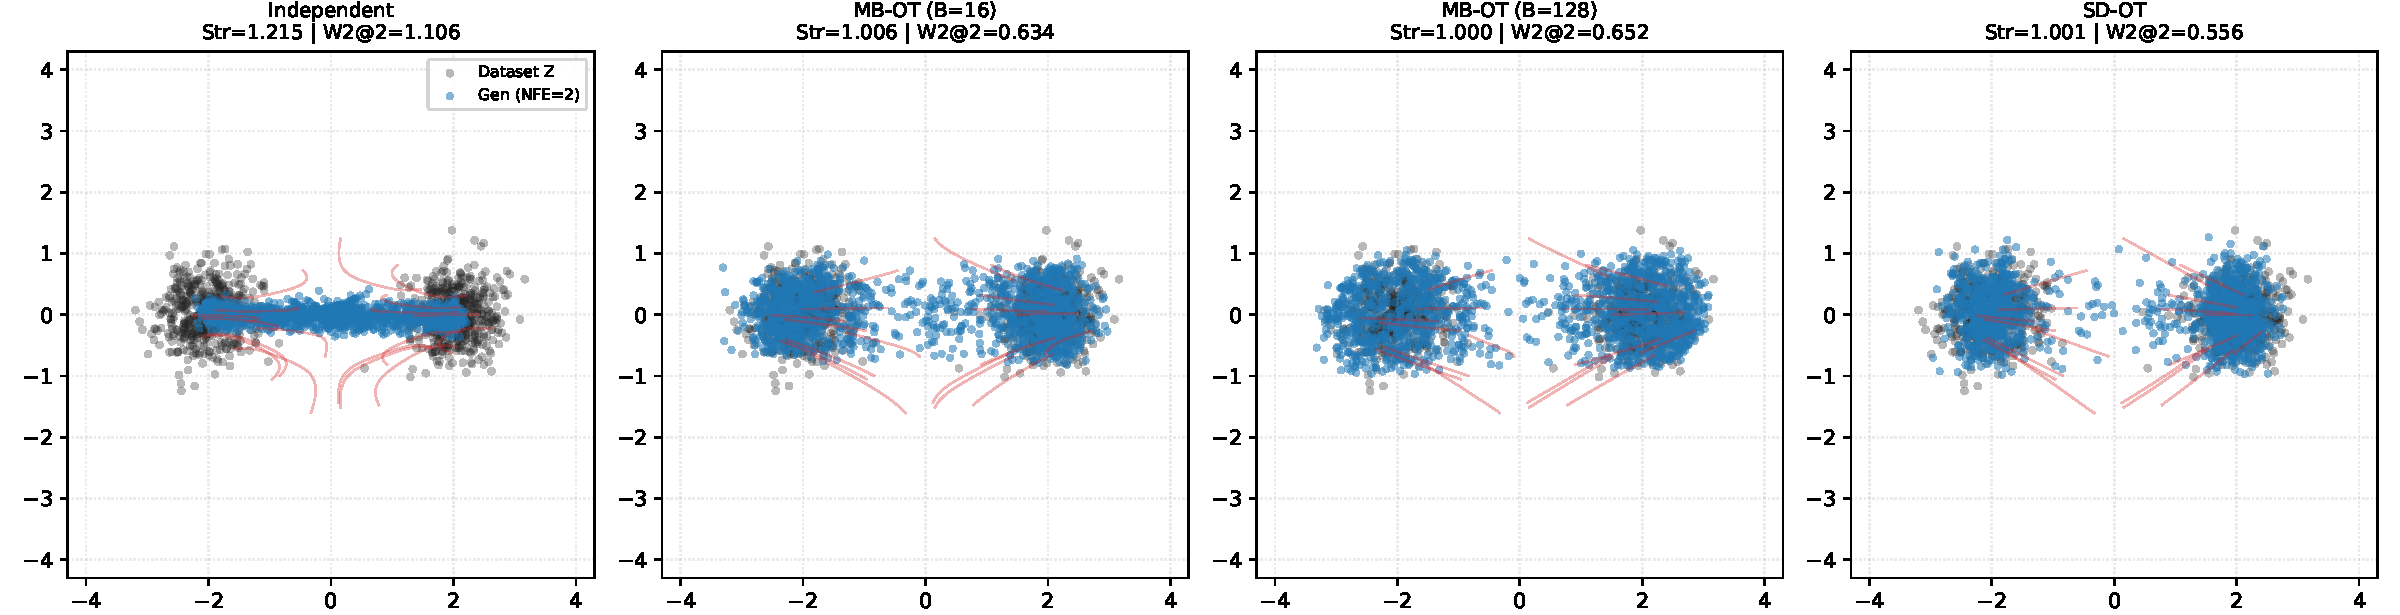
\includegraphics[width=0.96\textwidth]{sections/images/bimodal_N1024_nfe2.pdf}
        \caption{\texttt{Bimodal}}
    \end{subfigure}
    \vspace{0.3em}
    \begin{subfigure}[b]{\textwidth}
        \centering
        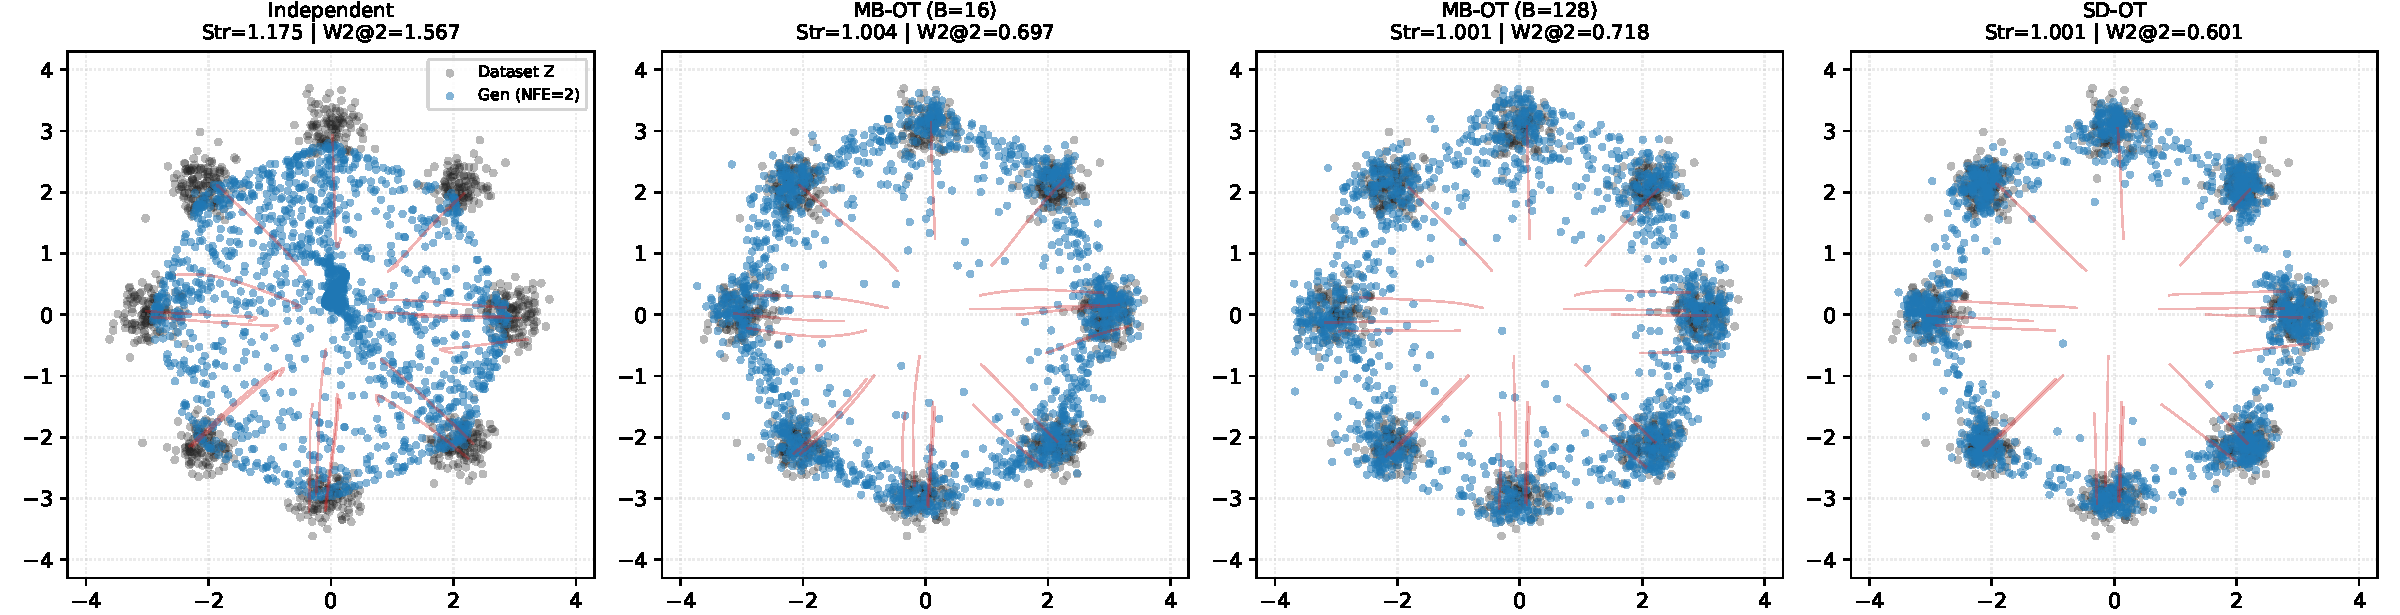
\includegraphics[width=0.96\textwidth]{sections/images/8_gaussians_N1024_nfe2.pdf}
        \caption{\texttt{8\_Gaussians}}
    \end{subfigure}
    \vspace{0.3em}
    \begin{subfigure}[b]{\textwidth}
        \centering
        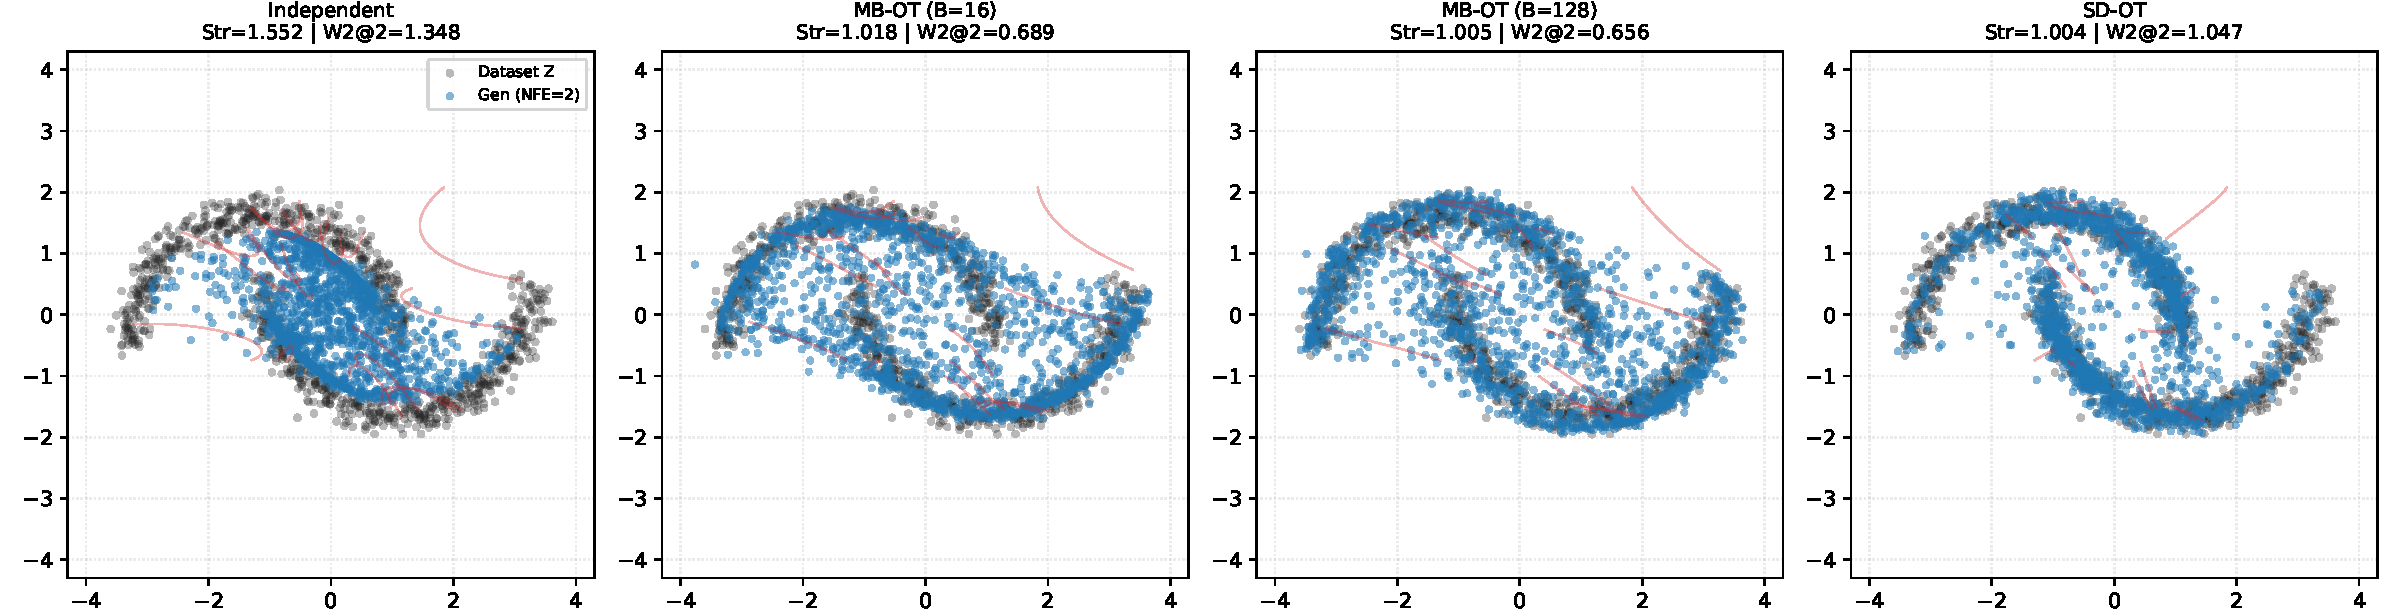
\includegraphics[width=0.96\textwidth]{sections/images/two_moons_N1024_nfe2.pdf}
        \caption{\texttt{Two\_Moons}}
    \end{subfigure}
    \vspace{0.3em}
    \begin{subfigure}[b]{\textwidth}
        \centering
        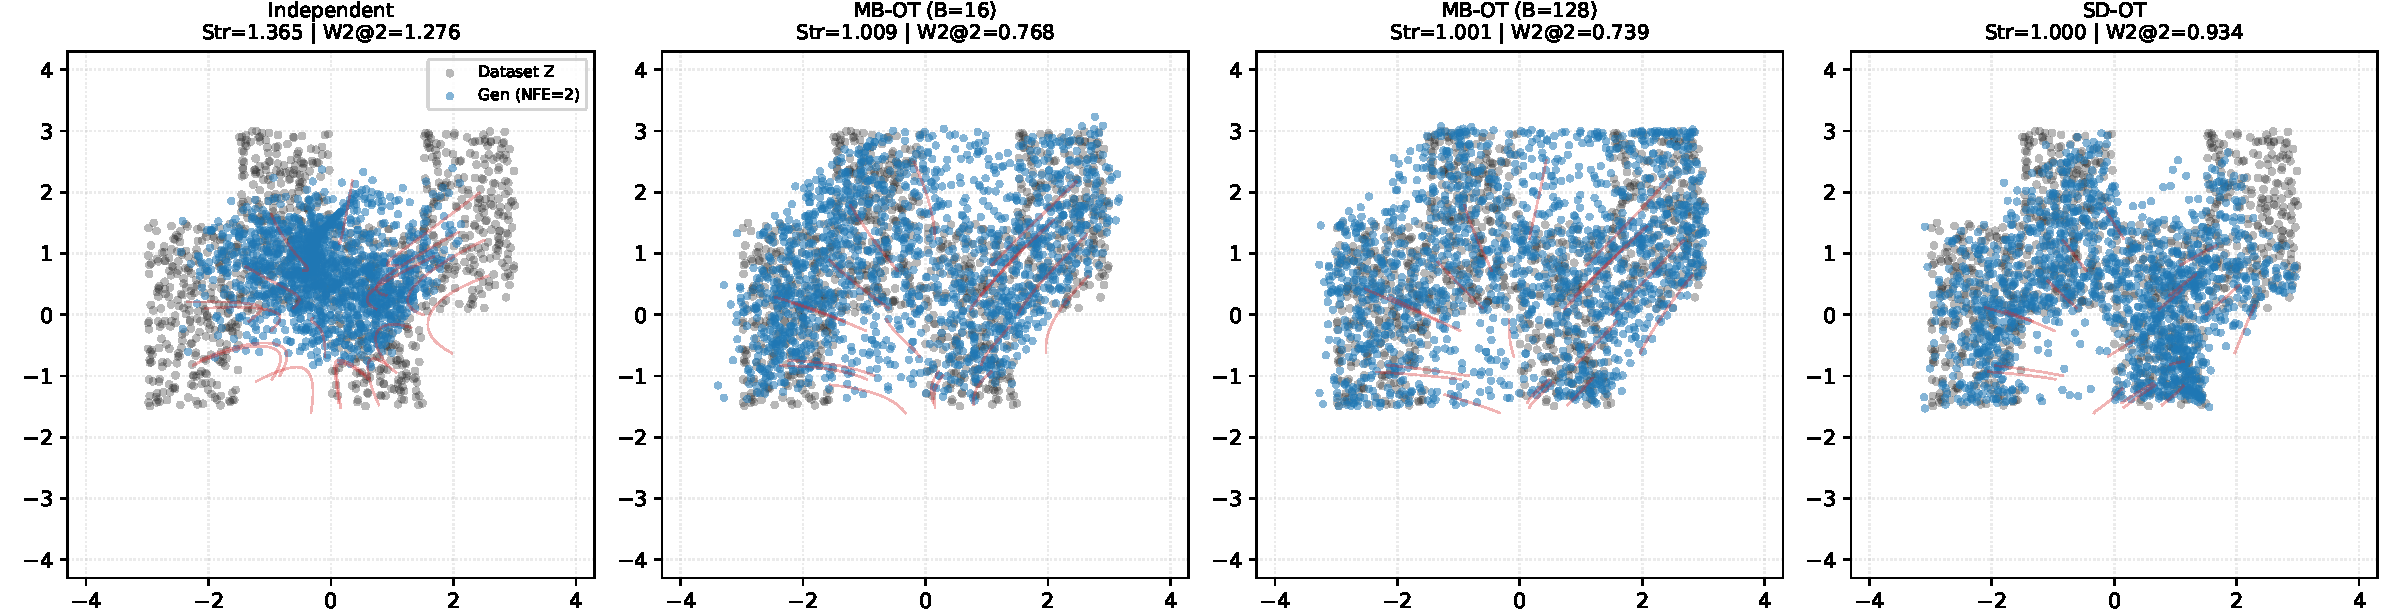
\includegraphics[width=0.96\textwidth]{sections/images/checkerboard_N1024_nfe2.pdf}
        \caption{\texttt{Checkerboard}}
    \end{subfigure}
    \caption{Qualitative comparison at $\text{NFE}=2$ across all four benchmarks ($N=1024$). Black dots denote the empirical target set $Z$, blue dots indicate generated samples after two Euler steps, and red curves trace learned ODE trajectories.}
    \label{fig:nfe2_qualitative}
\end{figure*}

\subsection{Sample Quality vs. NFE}

Figure~\ref{fig:w2_curves} tracks the empirical $W_2$ distance as the number of Euler steps increases from $\text{NFE}=1$ to $\text{NFE}=50$. Across all datasets, the independent coupling requires significantly more steps to converge, whereas OT-based couplings achieve near-optimal $W_2$ within one or two steps, resulting in nearly flat error curves. At $\text{NFE}=50$, however, the independent coupling remains fully competitive---achieving the lowest $W_2$ on \texttt{Two\_Moons} and \texttt{Checkerboard}, and matching SD-OT on \texttt{Bimodal} ($0.5461$ vs.\ $0.5442$). This confirms that the primary benefit of OT couplings lies in few-step generation rather than asymptotic many-step accuracy. \todo{check this paragraph against the curves of Figure~\ref{fig:w2_curves}.}

An instructive failure mode appears on \texttt{Two\_Moons} and \texttt{Checkerboard}: although \textbf{SD-OT} drives $\mathcal{C}(\pi)$ down to $\approx 0.01$ and achieves near-unit straightness, its empirical $W_2$ degrades ($1.0468$ and $0.9344$) compared to \textbf{MB-OT ($B=128$)} ($0.6562$ and $0.7390$). We attribute this to two factors:
\begin{enumerate}
    \item \textbf{Boundary discontinuities:} Across Laguerre cell boundaries, nearby noise points jump to distant targets $z^{(i)}$, rendering the optimal velocity field discontinuous and difficult for a smooth neural network to approximate on non-convex or disconnected supports.
    \item \textbf{Dual potential mass imbalance:} Because the dual potentials $v^*$ are estimated numerically, the resulting cell masses only approximate $1/N$, causing certain target points $z^{(i)}$ to be over- or under-sampled. \todo{report the cell-mass error $N \max_i |P_i - 1/N|$ of the learned potentials to decide between both hypotheses.}
\end{enumerate}

A natural way to alleviate these boundary discontinuities is to replace the hard Laguerre assignment with a soft probabilistic assignment based on distance to the cell boundaries. Specifically, replacing the $\arg\min$ with a softmax over the dual scores assigns each $x_0 \sim p_0$ to $z^{(i)}$ with probability
\begin{equation}
    w_i(x_0) = \frac{\exp\big((v_i - \|x_0 - z^{(i)}\|^2)/\varepsilon\big)}{\sum_{k=1}^N \exp\big((v_k - \|x_0 - z^{(k)}\|^2)/\varepsilon\big)},
\end{equation}
where the potentials $v$ are calibrated so that each target point receives uniform marginal mass $1/N$. This corresponds to entropically regularized semi-discrete OT, where $\varepsilon > 0$ interpolates smoothly between exact SD-OT ($\varepsilon \to 0$) and the independent coupling ($\varepsilon \to \infty$), yielding a smooth optimal vector field with full path support at the cost of a small nonzero $\mathcal{C}(\pi_\varepsilon)$. We leave an empirical study of this regularized variant to future work. \todo{decide whether to include an experiment varying $\varepsilon$.}


\begin{figure*}[t]
    \centering
    \begin{subfigure}[b]{0.48\textwidth}
        \centering
        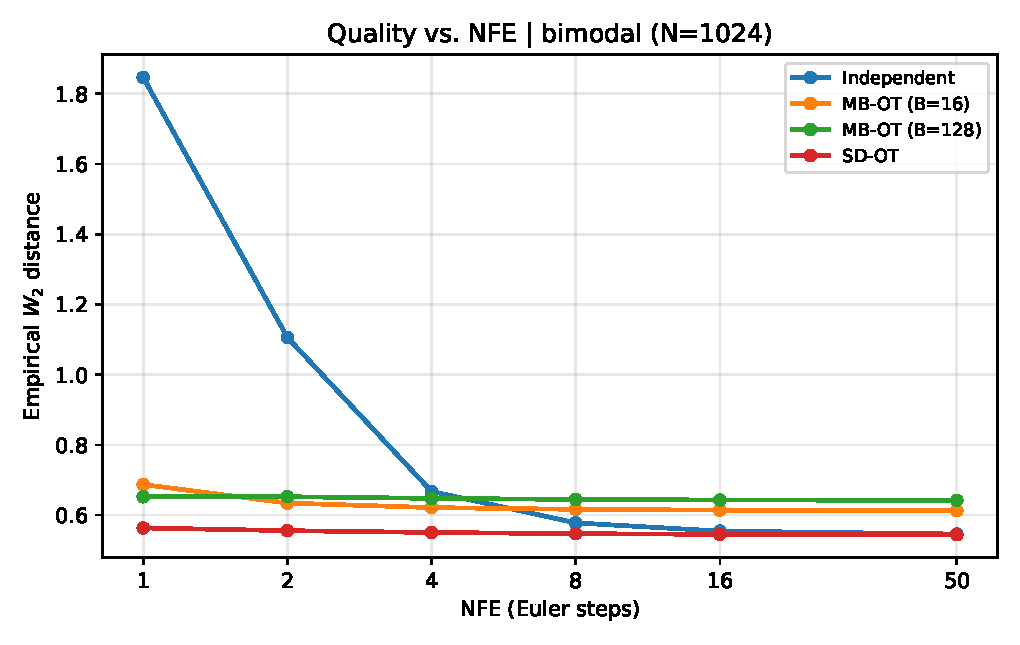
\includegraphics[width=\textwidth]{sections/images/bimodal_N1024_w2_curve.pdf}
        \caption{\texttt{Bimodal}}
    \end{subfigure}
    \hfill
    \begin{subfigure}[b]{0.48\textwidth}
        \centering
        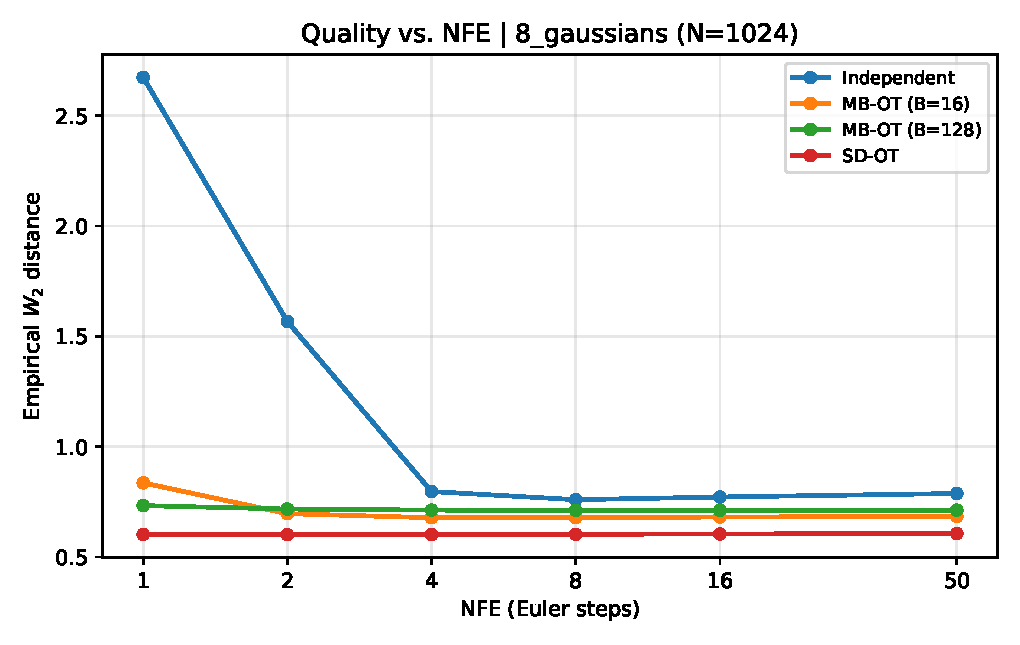
\includegraphics[width=\textwidth]{sections/images/8_gaussians_N1024_w2_curve.pdf}
        \caption{\texttt{8\_Gaussians}}
    \end{subfigure}
    
    \vspace{0.6em}
    
    \begin{subfigure}[b]{0.48\textwidth}
        \centering
        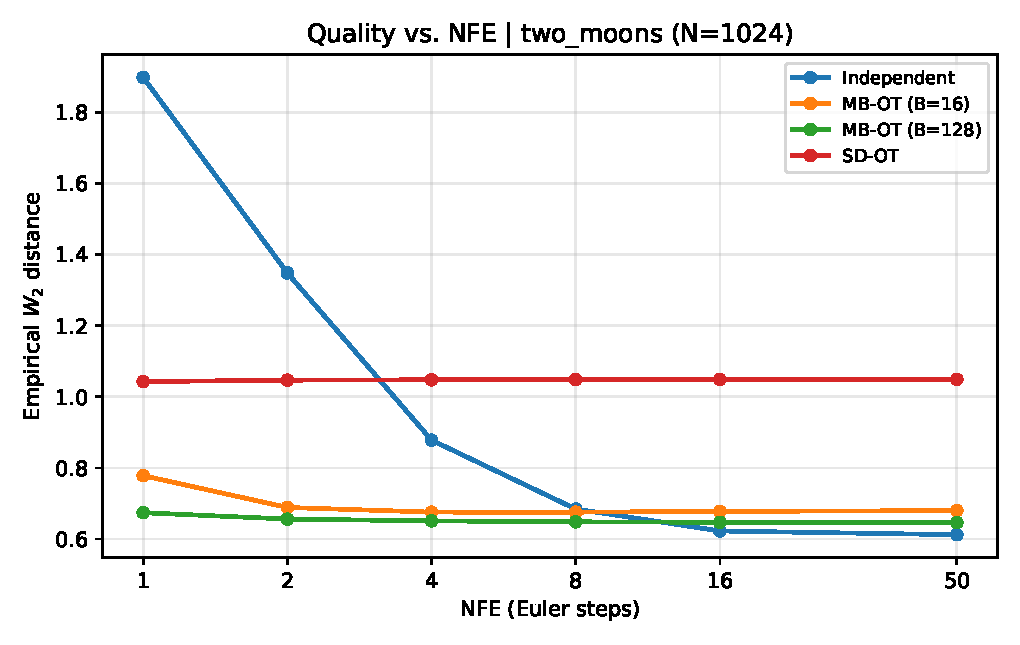
\includegraphics[width=\textwidth]{sections/images/two_moons_N1024_w2_curve.pdf}
        \caption{\texttt{Two\_Moons}}
    \end{subfigure}
    \hfill
    \begin{subfigure}[b]{0.48\textwidth}
        \centering
        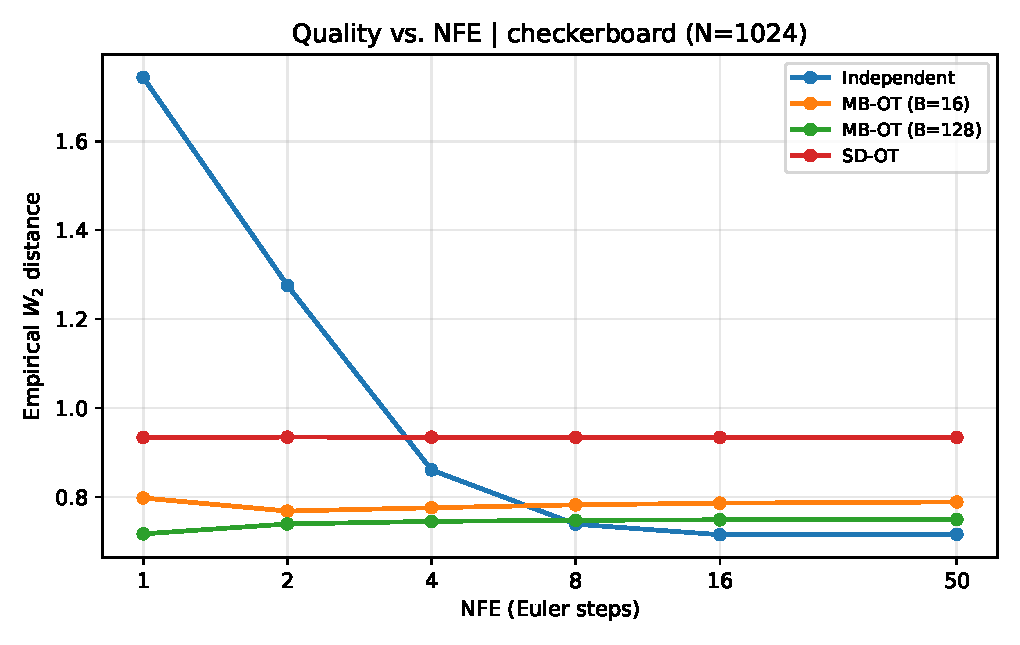
\includegraphics[width=\textwidth]{sections/images/checkerboard_N1024_w2_curve.pdf}
        \caption{\texttt{Checkerboard}}
    \end{subfigure}
    \caption{Empirical $W_2$ distance as a function of the number of function evaluations (NFE) on a logarithmic scale.}
    \label{fig:w2_curves}
\end{figure*}

Overall, \textbf{MB-OT ($B=128$)} offers the best practical trade-off: it reduces $\mathcal{C}(\pi)$ from $[3.43, 5.88]$ down to $\approx 0.14\text{--}0.19$, runs in under $10\,\text{s}$ ($20\times$ faster than SD-OT), preserves uniform target marginals by construction without dual optimization instability, and delivers strong two-step sample quality across all four geometries. Even a modest batch size (\textbf{MB-OT ($B=16$)}) already captures most of the straightness gains over independent Flow Matching.